\section{Problema 2: Algo Rush}

\subsection{Descripción de la problemática}
En este caso, se tiene un edificio con N pisos y con pasillos de longitud L y existen portales bidireccionales que comunican dos puntos determinados del mismo. Utilizar un portal consume dos segundos y caminar un metro consume un segundo. Se sabe que no hay más de un portal que comunique las mismas posiciones del mismo par de pisos.
Se requiere un algoritmo que determine la cantidad minima de segundos en ir desde el inicio del piso 0 hasta el final del último piso.

\subsection{Resolución propuesta y justificación}
Lo primero que hace el algoritmo es transformar la entrada en un grafo. Según nuestra representación, cada portal es considerado como un nodo. Las aristas que parten de un nodo llegan a todos aquellos otros nodos a los que se puede alcanzar desde el actual, ya sea porque son un punto de destino de teletransporte del mismo, o porque se encuentran en el mismo piso y se puede alcanzar caminando.

Como estructura auxiliar para construir el grafo se utiliza un diccionario de diccionarios de nodos, cuyas claves para acceder a un nodo son el piso y la distancia respectivamente. Como en este caso las claves son enteros, y comprenden el rango de 0 a N para el primero, y de 0 a L para los subdiccionarios, se ha implementodo un diccionario al que llamamos BoundedIntegerMap, que construye un array de elementos con un largo especificado en el constructor y, para acceder a la definición de una clave, accede a la posición del array que corresponde a la clave. De esta forma, la lectura y escritura a un BoundedIntegerMap es O(1).
Un nodo contiene: un identificador (un int propio de cada nodo), la posicion en el pasillo donde se encuentra, un conjunto de nodos a los cuales se puede llegar caminando y un conjunto de nodos que son puntos de destino de teletransporte.

Posterirmente un segundo algoritmo, utilizando el grafo generado por el primero, se encarga de determinar el camino entre ambos extremos del grafo (desde el principio del piso 0 hasta el final del último piso, basadose en el BFS relajando ejes. El BFS se utiliza para calcular caminos mínimos en ejes sin peso; para esto, determina en cada paso la distancia al inicio de todos los adyacentes a determinado nodo X, considerando que, o bien el camino mínimo desde la raiz hasta el nodo evaluado pasaba por X, por lo cual es el camino mínimo hasta X más uno, o existía un camino más rapido hasta el nodo, pero entonces, el mismo ya se habrá evaluado anteriormente, por lo cual ya se conocerá el camino mínimo. El BFS relajando ejes consiste en adaptar un grafo pesado para simular un grafico sin pesos en aristas. Para esto, cuando una aristaa contiene un peso superior a 1, coloca nodos ``fantasma'' entre ambos para aumentar la distancia entre los nodos.
El algoritmo utilizado en el TP utiliza una cola en donde ingresa los adyacentes de los nodos evaluados para procesarlos luego de forma ordenada. Para emular los nodos fantasma, el algoritmo crea un solo nodo extra, que almacena la cantidad de nodos fantasma que deberían existir, y, si el algoritmo detecta que el nodo evaluado emula a más de un fantasma, altera dicho valor y lo vuelve a encolar.

\subsection{Análisis de la complejidad}
Inicialmente, se debe construir un BoundedIntegerMap de N elementos y luego N BoundedIntegerMap de L elementos, lo cual tiene un costo de O(NL). Luego se procesa la entrada que determina las posiciones de los portales y se van creando los nodos y clasificando en los BoundedIntegerMap. Como la consulta y escritura en el BoundedIntegerMap es O(1), la complejidad total es de O(P). Finalmente, la complejidad de formar el grafo es de O(P+NL).
Luego comienza a ejecutarse el algoritmo que calcula el camnino mínimo. En el peor caso, el algoritmo debe recorrer cada uno de los nodos. Sabemos que el grafo no tiene más de N*L + P nodos,incluyendo los nodos fantasma, ya que dos nodos calificados en un mismo piso no pueden estar separados por una distancia superior a L; además, se debe agregar un nodo fantasma para marcar el paso de un nodo a otro por teletransporte, por lo cual existen P nodos fantasma extra. Entonces, la complejidad del algoritmo de camino mínimo es O(NL).
Finalmente, el costo de construir el grafo y hallar el camino mínimo entre sus extremos es O(P+ NL).

\subsection{Código fuente}
A continuación se incluyen las partes más relevantes del código.
La clase \emph{Lector.java} se encarga de tomar los datos del archivo de entrada y procesarlos para construir el grafo.
\lstinputlisting[name=pp, numbers=left, frame=lines, firstline=51, lastline=129]{../src/ej2/src/Lector.java}
La clase \emph{Solucion.java} contiene los métodos que calculan el camino mínimo del grafo entre los dos puntos señalados.
\lstinputlisting[name=pp, numbers=left, frame=lines, firstline=14, lastline=76]{../src/ej2/src/Solucion.java}

\subsection{Experimentación}

\subsubsection{Piensa con portales}
En este test existe un portal que lleva diréctamente desde la entrada al aula. El algoritmo debería utilizarlo y llegar al aula en dos segundos.

\subsubsection{Encontre un atajo}
En este test existen dos portales en el primer piso con una longitud considerable. El primero de ellos toma un camino largo hacia el aula y el otro uno más corto. Como debido a la distancia entre el origen de ambos caminos, el algoritmo comenzará a adentrarse en el camino largo antes del corto. Se pretende testear si el algoritmo finalmente devuelve la solución correcta a pesar de esto.

\subsubsection{¿y_como_llegue_aqui?}
En esta oportunidad se introduce un ciclo en el grafo. Existen dos portales en el piso cero, uno de los cuales entra al ciclo y otro que lleva a la dirección correcta.

\subsubsection{Linea recta}
Este test se basa en probar la correctitud algoritmo cuando existen portales superpuestos. Existe un único camino entre el inicio y el aula, en donde todos los portales intermedios tienen otro superpuesto que lleva a otro piso, por lo que no es necesario camninar, excepto en el primer y el último piso.

\subsubsection{cuello_botella}
Este test tambíen esta centrado en probar el algoritmo cuando existen portales superpuestos. En este caso, existen muchos portales con un extremo en un mismo punto.

\subsubsection{No quiero caminar}
Este test se centra en explotar la posibilidad de utilizar un portal que comunica dos puntos del mismo piso. En él, existen dos pisos con un portal en cada extremo y se necesita llegar de uno a otro dentro de cualquier camino existente; sin embargo, otro portal que cuyos extremos son muy cercanos a cada uno de los portales, por lo cual el camino mínimo deberia utilizar estos portales intermedios.

\subsubsection{la_venganza_de_los_ciclos}
En la entrada de este test se presentan dos ciclos en el grafo; dentro del camino mínimo se incluyen algunos nodos pertenecientes a los mismos. Nuevamente se pretende evaluar el comportamiento del algoritmo frente a los ciclos, pero en esta ocasión incluyéndolos dentro de un camino simple hasta el aula.

\subsubsection{salidas_de_emergencia}
En esta oportunidad se prueba el uso intensivo de nodos fantasma. En este test sólo existen portales que comunican el principio de un piso con el final del piso anterior.

\subsubsection{Constrastación Empírica de la complejidad}
Para poner a prueba de manera empirica la complejidad algorítmica calculada para nuestra resolución, diseñamos tres casos distintos de pruebas:
\begin{itemize}
\item{Caso en el que se incrementa la cantidad de portales, dejando fijos los valores de la cantidad de pisos y la longitud de los pasillos.}
\item{Caso en el que se incrementa la cantidad de pisos, dejando fijos los valores de la cantidad de portales y la longitud de los pasillos.}
\item{Caso en el que se incrementa la longitud de los pasillos, dejando fijos los valores de la cantidad de pisos y la cantidad de portales.}
\end{itemize}

Estos casos fueron diseñados partiendo del análisis de la complejidad dada. Siendo la misma O(NL+P), dedujimos que tomando como variable sólo una de ellas de manera alternada en tres casos distintos, se podrían obtener las funciones \textit{ f(N) = a*N + b},  \textit {f(L) = a*L + b} y \textit{f(P) = b + P}, todas ellas lineales. \\

A continuación se pueden ver, en las figuras \ref{pisos}, \ref{pasillos} y \ref{portales} los resultados de las mediciones de tiempos obtenidas a partir de grafos válidos  generados de forma automática para cada caso en particular.


\begin{figure}[h!]
   \begin{center}
 	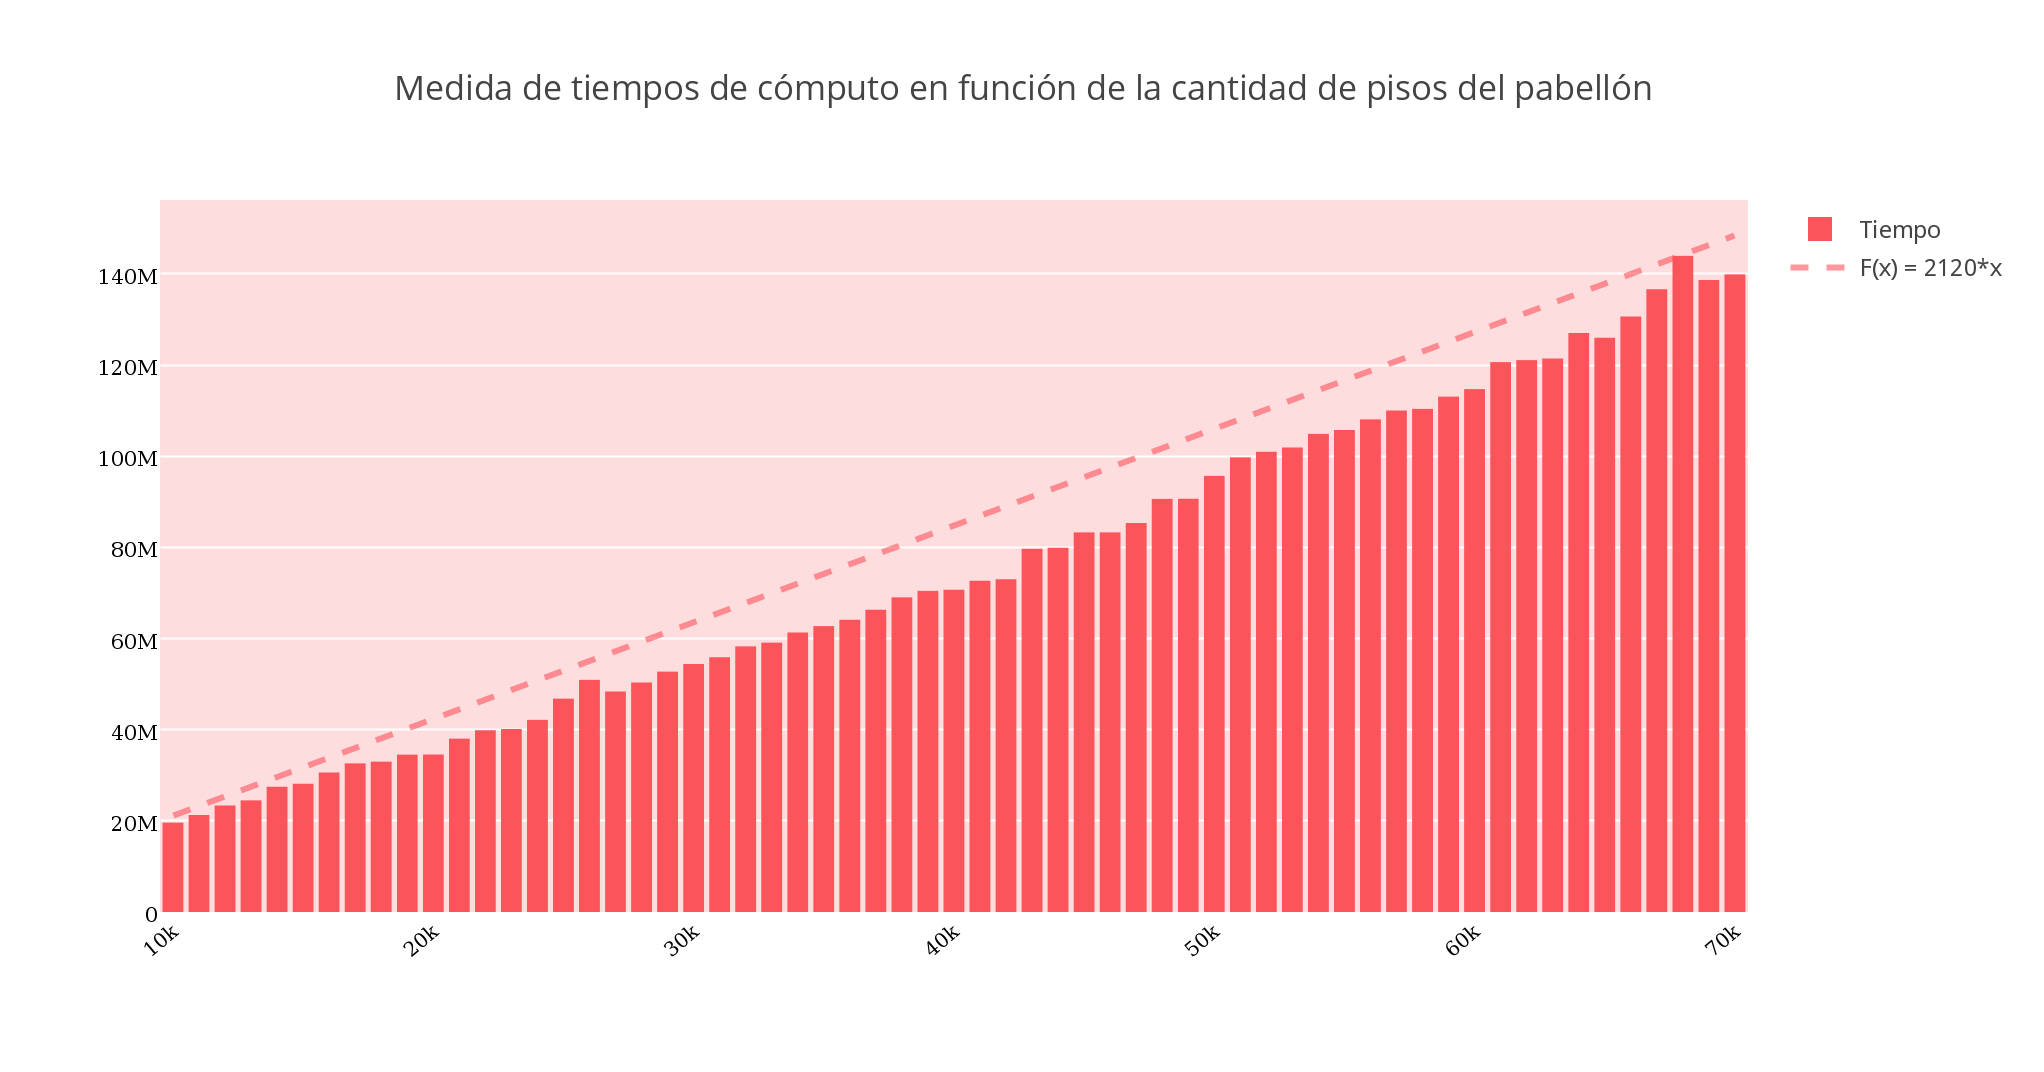
\includegraphics[width=18cm]{imagenes/ej2/f(pisos).png}
	\caption{Medición de tiempos en función de la cantidad de pisos}
	\label{pisos}
   \end{center}
 \end{figure}

 \begin{figure}[h!]
   \begin{center}
 	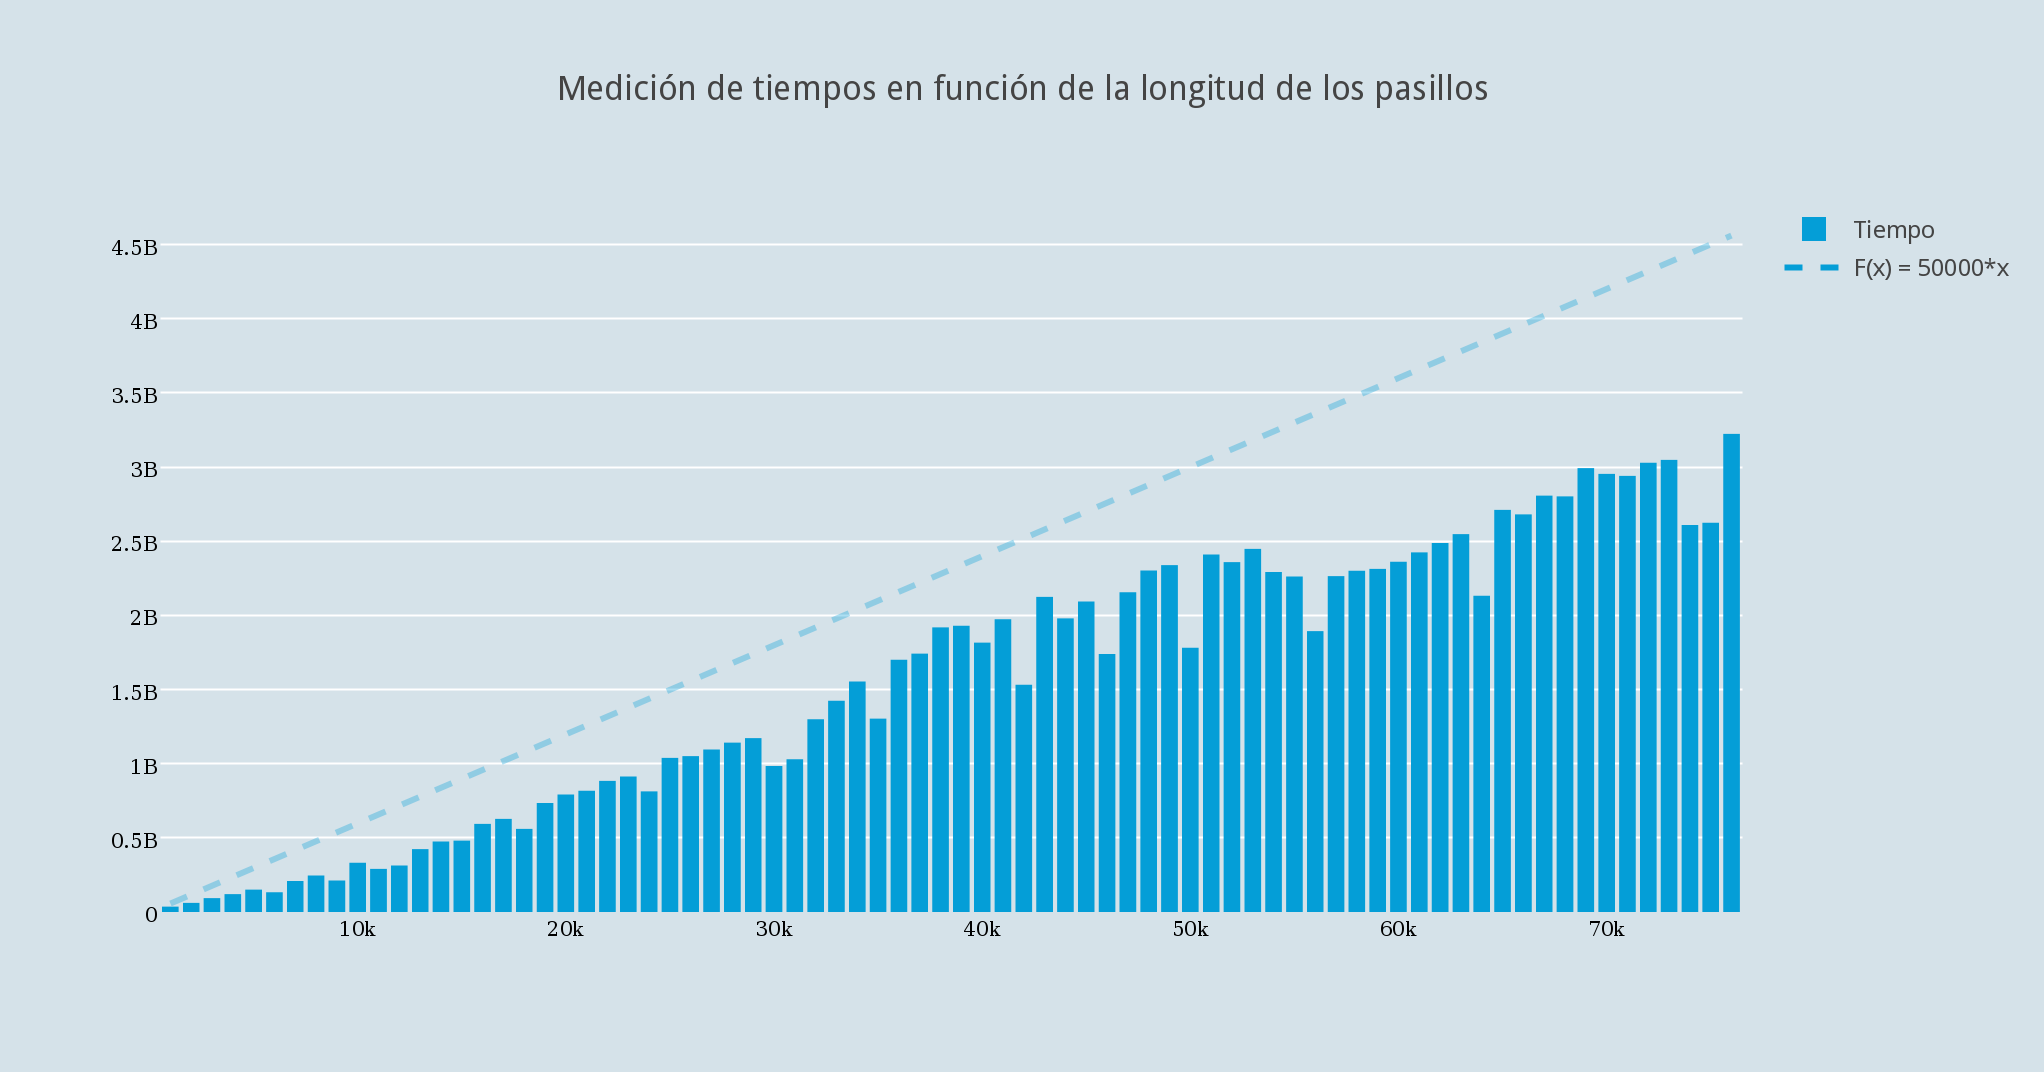
\includegraphics[width=18cm]{imagenes/ej2/f(pasillos).png}
	\caption{Medición de tiempos en función de la longitud de los pasillos}
	\label{pasillos}
   \end{center}
 \end{figure}

\begin{figure}[h!]
   \begin{center}
 	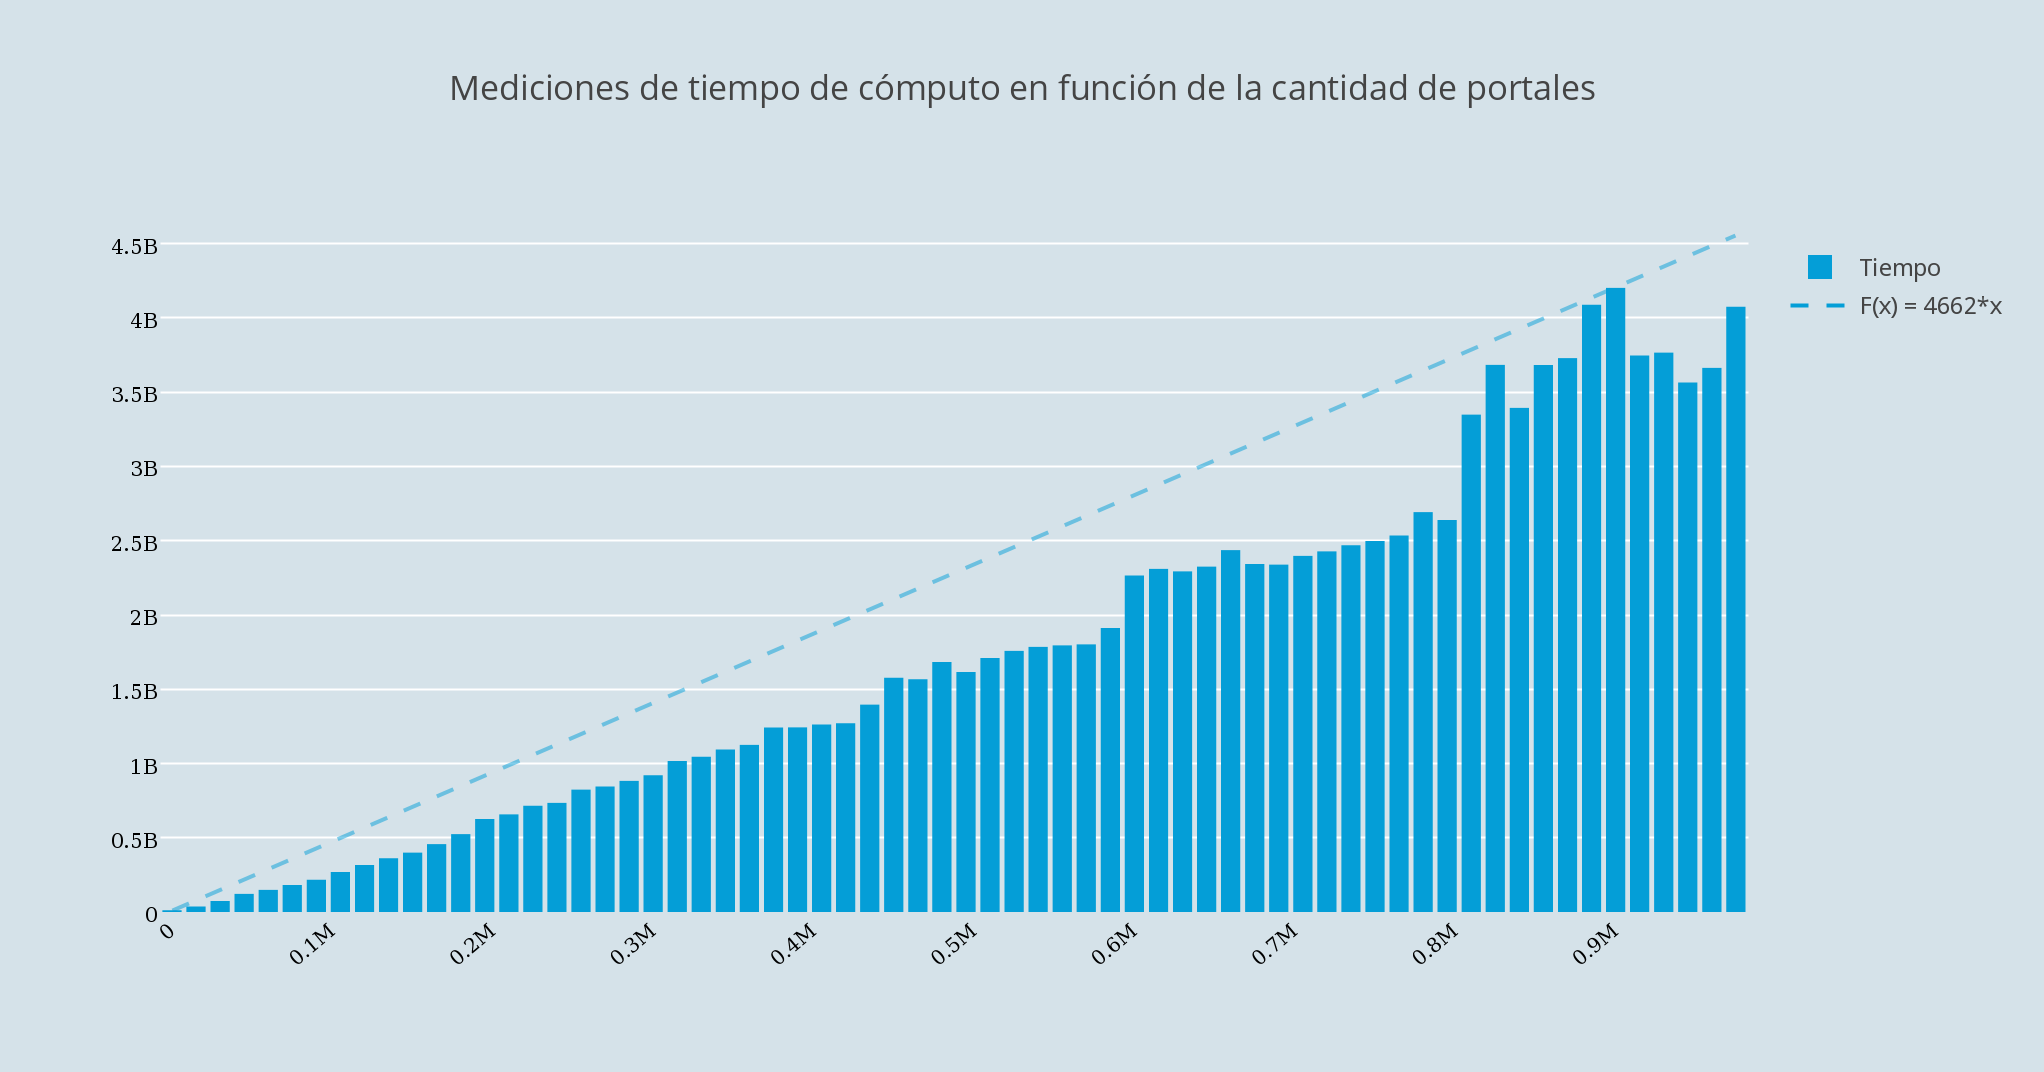
\includegraphics[width=18cm]{imagenes/ej2/f(portales).png}
	\caption{Medición de tiempos en función de la cantidad de portales}
	\label{portales}
   \end{center}
 \end{figure}


Como es posible observar, los tiempos medidos en cada uno de los casos parecen comportarse de forma tal que su crecimiento fuera lineal en función de la variable escogida.\\

Si bien tenemos presente que hacer estas pruebas no garantiza la reconstrucción de la complejidad O(NL+P) (del mismo modo que ninguna prueba empírica de este estilo \textit{prueba} de ninguna manera una determinada complejidad temporal) consideramos que las experimentaciones expuestas ayudan a reforzar en cierta medida los resultados teóricos deducidos a priori. \\

\subsubsection{Peor caso}
Como mencionamos anteriormente, el grafo generado a partir de la entrada no puede tener más de NL+P nodos. Sin embargo, en algunas ocasiones este máximo no es alcanzado, ya que, aquellos pisos que no posean nodos en los extremos aportarán menos de L nodos al grafo. Entonces, la entrada generada como peor caso sólo tiene portales en los extremos de los pisos, de forma tal que se comunique el final de un piso i con el principio del piso i+1. De esta forma el grafo siempre tiene NL + P nodos. Para mantener estas proporciones, en este test cambian dos variables a la vez: cada vez que se añade un piso se agrega también un nuevo portal desde el final de dicho piso al principio del siguiente. La longitud de los pasillos se ha dejado fija en 400.\\
En la figura \ref{peorCaso} se pueden ver los resultados obtenidos luego de medir los tiempos de cómputo de una serie de grafos generados de manera tal que respeten la estructura descripta en este apartado.

\begin{figure}[h!]
   \begin{center}
 	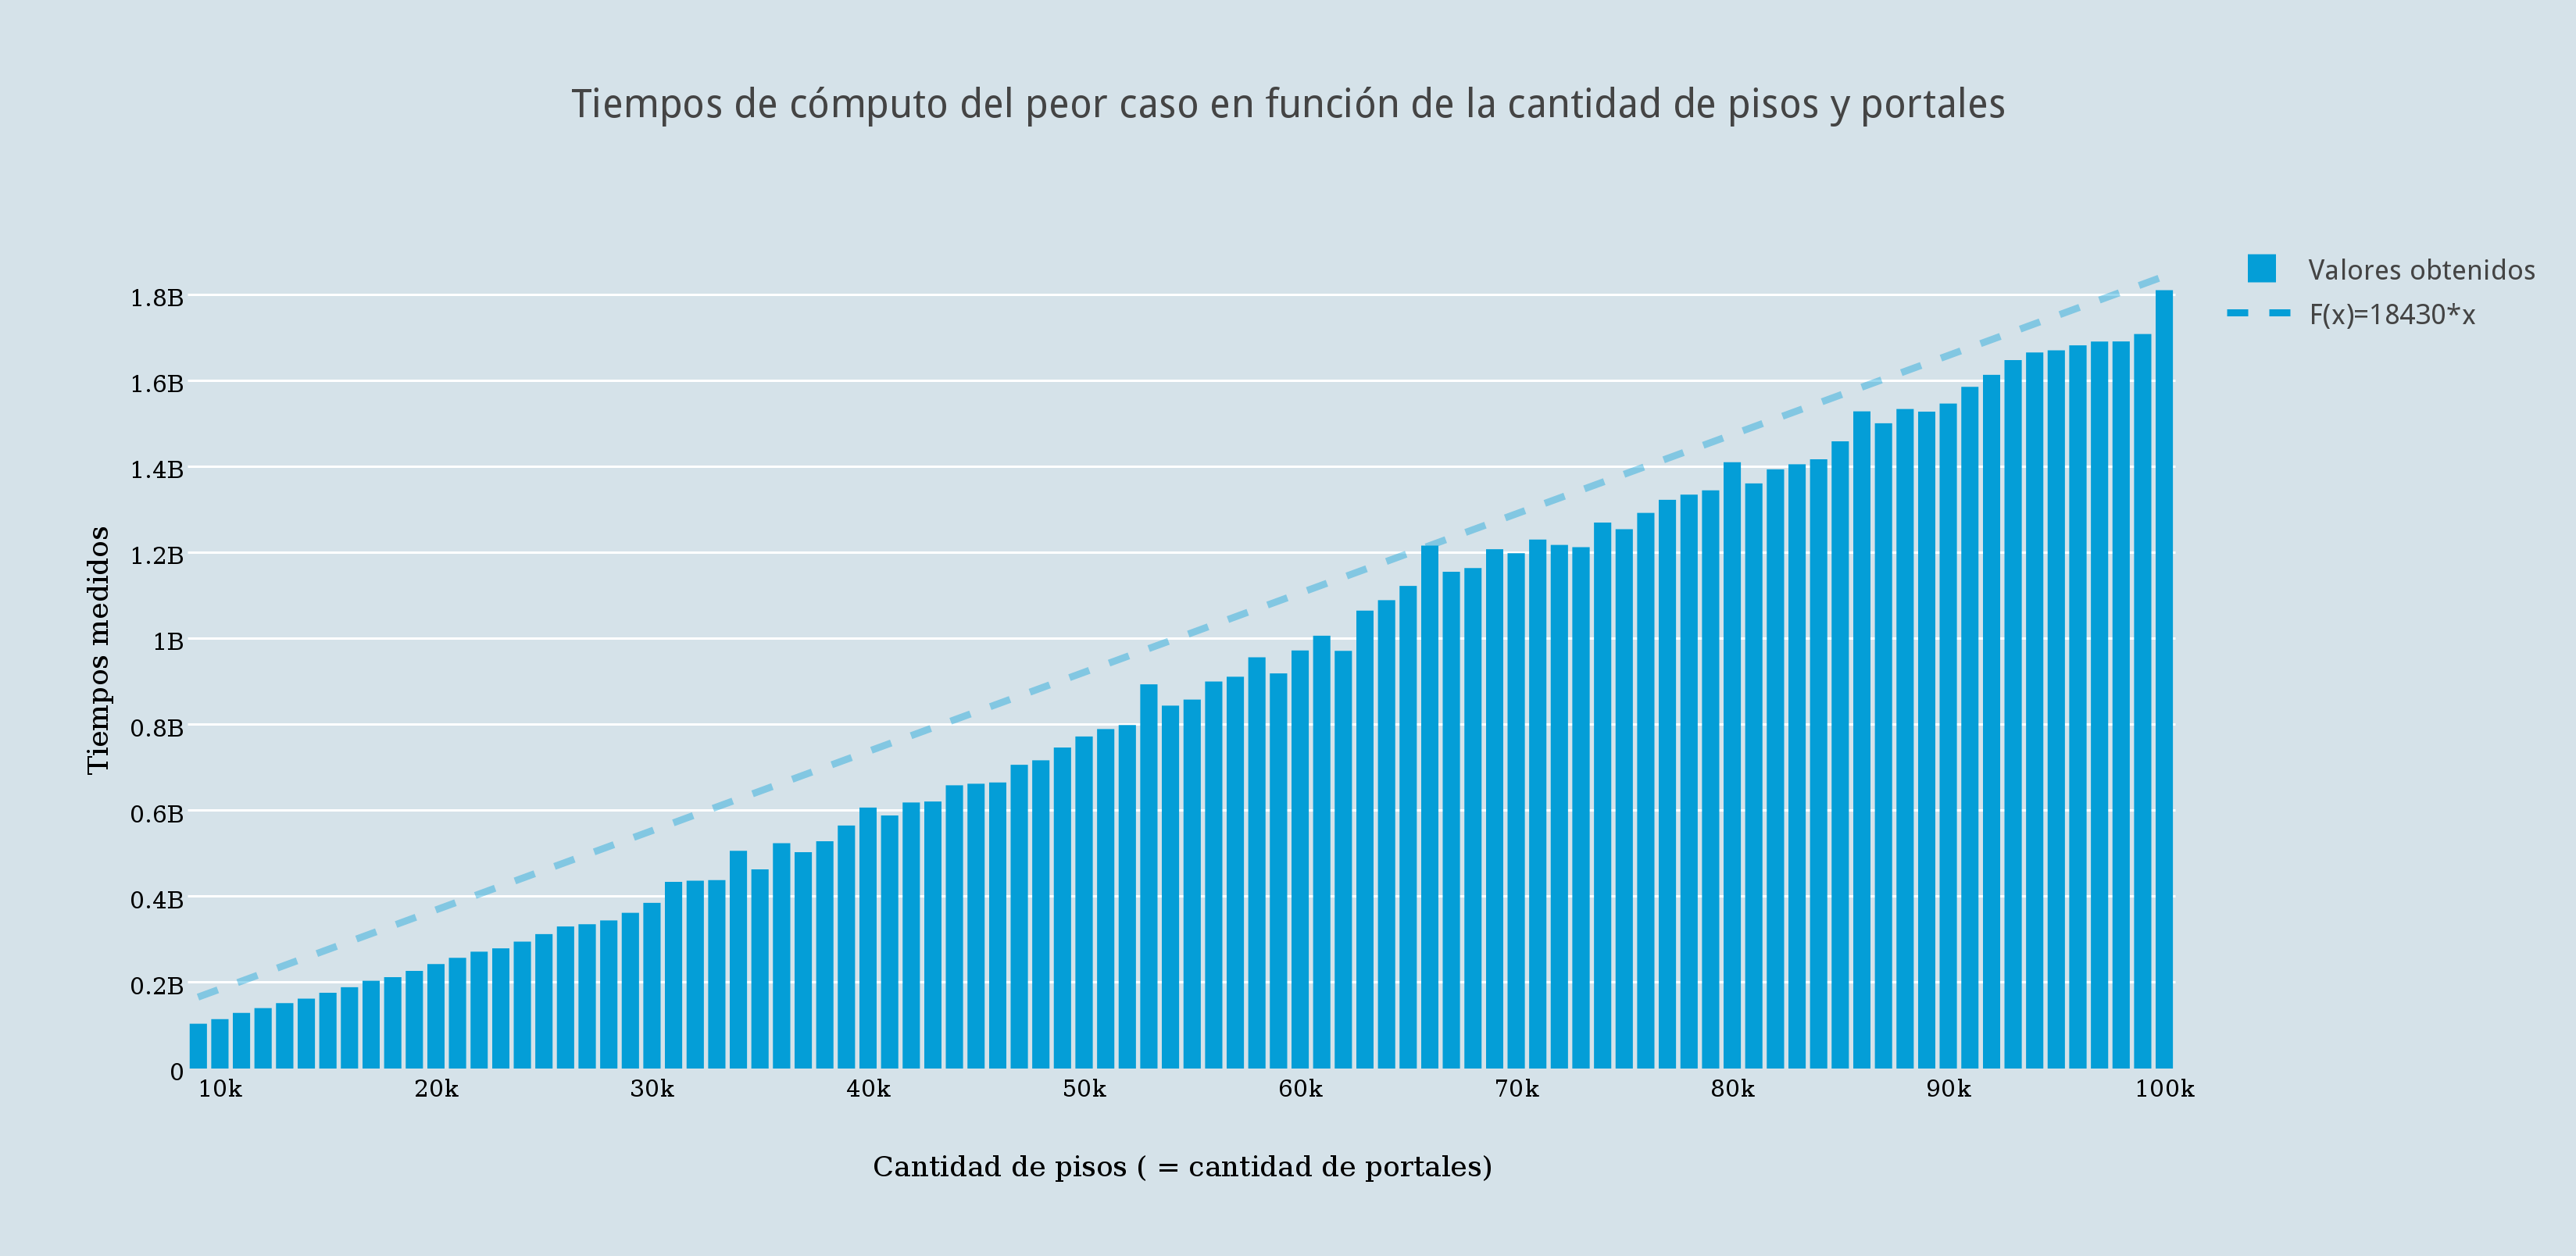
\includegraphics[width=18cm]{imagenes/ej2/peorCaso.png}
	%\caption{}
	\label{peorCaso}
   \end{center}
 \end{figure}


\subsubsection{Mejor caso}
En este caso sólo existe un portal entre el principio del primer piso hasta el final del último (es decir, el aula). En cada iteración la cantidad de pisos se incrementa. En este caso, la mayoría de los pisos están vacios y no aportarán nodos al mapa. Además, como los nodos del portal están superpuestos con los nodos de la entrada y del aula, el primer y el último piso tampoco aportarán nodos fantasma que dependan de la longitud. Sin embargo, al procesar la infomación de entrada, el Lector necesita chequear todos los pisos, por lo que, en el mejor caso, el tiempo de computo del Lector depende de N, aunque encontrar la solución al grafo no lo haga.\\
En la figura \ref{mejorCaso} se pueden observar los resultados obtenidos a través de la medición de tiempos para grafos de distinta cantidad de pisos que respetan la estructura descripta en este apartado.

\begin{figure}[h!]
   \begin{center}
 	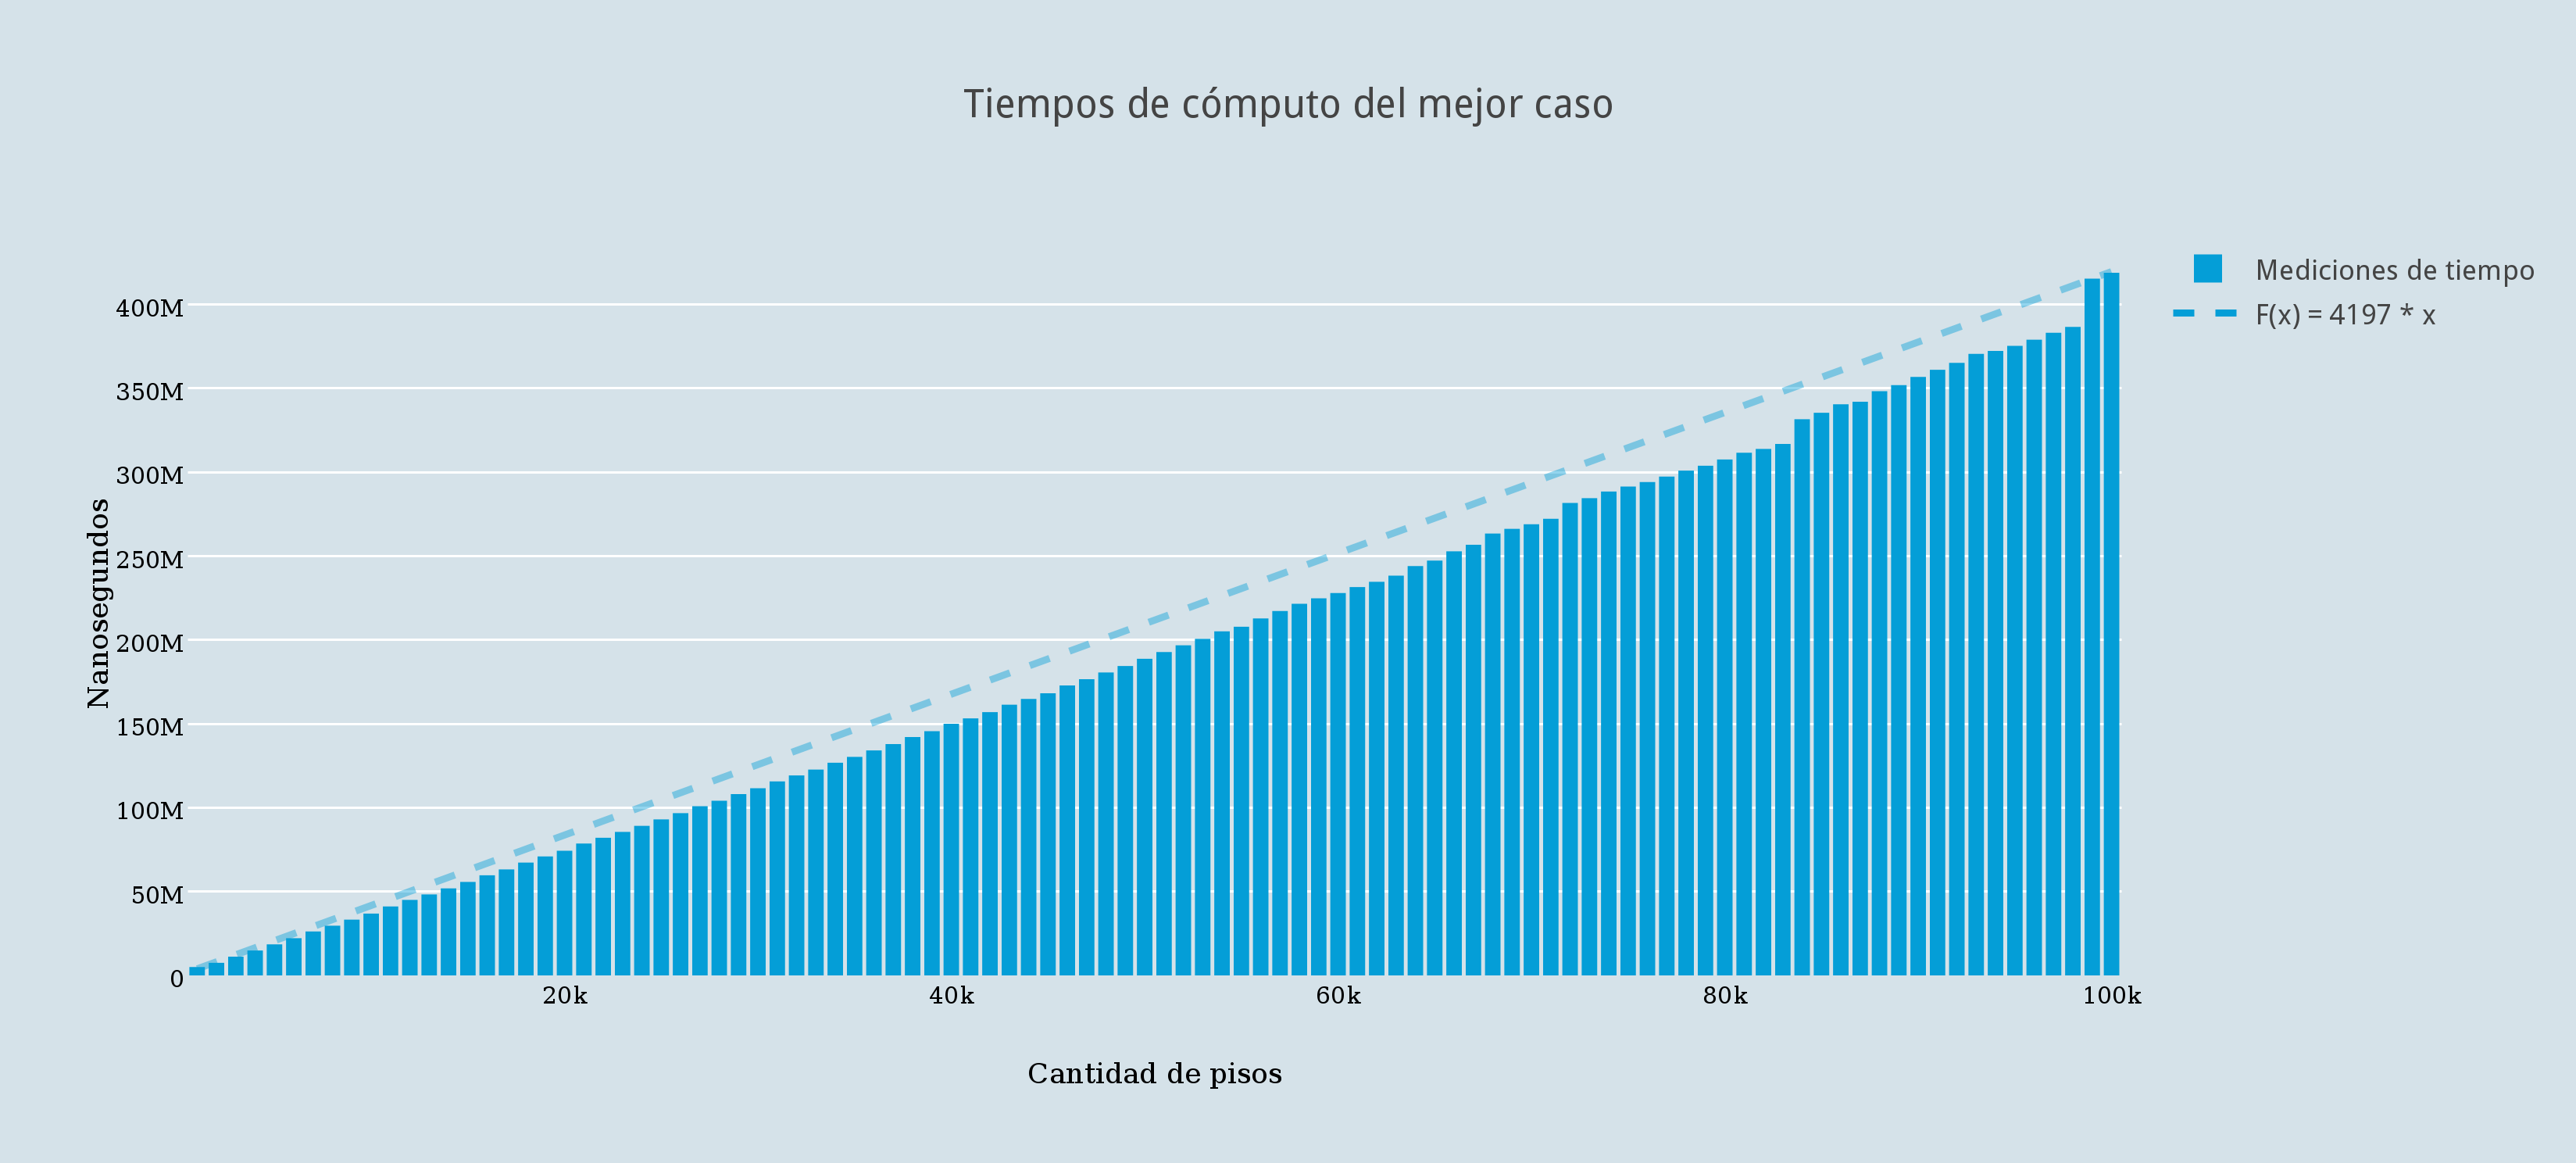
\includegraphics[width=18cm]{imagenes/ej2/mejorCaso.png}
	%\caption{}
	\label{mejorCaso}
   \end{center}
 \end{figure}

 Finalmente, en la figura \ref{comparativa} se puede apreciar la notoria diferencia entre los tiempos conseguidos por los peores casos respecto de los alcanzados por los mejores casos frente a la misma cantidad de pisos.


\newpage
